\documentclass[]{article}
\usepackage{lmodern}
\usepackage{amssymb,amsmath}
\usepackage{ifxetex,ifluatex}
\usepackage{fixltx2e} % provides \textsubscript
\ifnum 0\ifxetex 1\fi\ifluatex 1\fi=0 % if pdftex
  \usepackage[T1]{fontenc}
  \usepackage[utf8]{inputenc}
\else % if luatex or xelatex
  \ifxetex
    \usepackage{mathspec}
  \else
    \usepackage{fontspec}
  \fi
  \defaultfontfeatures{Ligatures=TeX,Scale=MatchLowercase}
\fi
% use upquote if available, for straight quotes in verbatim environments
\IfFileExists{upquote.sty}{\usepackage{upquote}}{}
% use microtype if available
\IfFileExists{microtype.sty}{%
\usepackage{microtype}
\UseMicrotypeSet[protrusion]{basicmath} % disable protrusion for tt fonts
}{}
\usepackage[margin=1in]{geometry}
\usepackage{hyperref}
\hypersetup{unicode=true,
            pdftitle={KC Housing Prices},
            pdfborder={0 0 0},
            breaklinks=true}
\urlstyle{same}  % don't use monospace font for urls
\usepackage{color}
\usepackage{fancyvrb}
\newcommand{\VerbBar}{|}
\newcommand{\VERB}{\Verb[commandchars=\\\{\}]}
\DefineVerbatimEnvironment{Highlighting}{Verbatim}{commandchars=\\\{\}}
% Add ',fontsize=\small' for more characters per line
\usepackage{framed}
\definecolor{shadecolor}{RGB}{248,248,248}
\newenvironment{Shaded}{\begin{snugshade}}{\end{snugshade}}
\newcommand{\KeywordTok}[1]{\textcolor[rgb]{0.13,0.29,0.53}{\textbf{#1}}}
\newcommand{\DataTypeTok}[1]{\textcolor[rgb]{0.13,0.29,0.53}{#1}}
\newcommand{\DecValTok}[1]{\textcolor[rgb]{0.00,0.00,0.81}{#1}}
\newcommand{\BaseNTok}[1]{\textcolor[rgb]{0.00,0.00,0.81}{#1}}
\newcommand{\FloatTok}[1]{\textcolor[rgb]{0.00,0.00,0.81}{#1}}
\newcommand{\ConstantTok}[1]{\textcolor[rgb]{0.00,0.00,0.00}{#1}}
\newcommand{\CharTok}[1]{\textcolor[rgb]{0.31,0.60,0.02}{#1}}
\newcommand{\SpecialCharTok}[1]{\textcolor[rgb]{0.00,0.00,0.00}{#1}}
\newcommand{\StringTok}[1]{\textcolor[rgb]{0.31,0.60,0.02}{#1}}
\newcommand{\VerbatimStringTok}[1]{\textcolor[rgb]{0.31,0.60,0.02}{#1}}
\newcommand{\SpecialStringTok}[1]{\textcolor[rgb]{0.31,0.60,0.02}{#1}}
\newcommand{\ImportTok}[1]{#1}
\newcommand{\CommentTok}[1]{\textcolor[rgb]{0.56,0.35,0.01}{\textit{#1}}}
\newcommand{\DocumentationTok}[1]{\textcolor[rgb]{0.56,0.35,0.01}{\textbf{\textit{#1}}}}
\newcommand{\AnnotationTok}[1]{\textcolor[rgb]{0.56,0.35,0.01}{\textbf{\textit{#1}}}}
\newcommand{\CommentVarTok}[1]{\textcolor[rgb]{0.56,0.35,0.01}{\textbf{\textit{#1}}}}
\newcommand{\OtherTok}[1]{\textcolor[rgb]{0.56,0.35,0.01}{#1}}
\newcommand{\FunctionTok}[1]{\textcolor[rgb]{0.00,0.00,0.00}{#1}}
\newcommand{\VariableTok}[1]{\textcolor[rgb]{0.00,0.00,0.00}{#1}}
\newcommand{\ControlFlowTok}[1]{\textcolor[rgb]{0.13,0.29,0.53}{\textbf{#1}}}
\newcommand{\OperatorTok}[1]{\textcolor[rgb]{0.81,0.36,0.00}{\textbf{#1}}}
\newcommand{\BuiltInTok}[1]{#1}
\newcommand{\ExtensionTok}[1]{#1}
\newcommand{\PreprocessorTok}[1]{\textcolor[rgb]{0.56,0.35,0.01}{\textit{#1}}}
\newcommand{\AttributeTok}[1]{\textcolor[rgb]{0.77,0.63,0.00}{#1}}
\newcommand{\RegionMarkerTok}[1]{#1}
\newcommand{\InformationTok}[1]{\textcolor[rgb]{0.56,0.35,0.01}{\textbf{\textit{#1}}}}
\newcommand{\WarningTok}[1]{\textcolor[rgb]{0.56,0.35,0.01}{\textbf{\textit{#1}}}}
\newcommand{\AlertTok}[1]{\textcolor[rgb]{0.94,0.16,0.16}{#1}}
\newcommand{\ErrorTok}[1]{\textcolor[rgb]{0.64,0.00,0.00}{\textbf{#1}}}
\newcommand{\NormalTok}[1]{#1}
\usepackage{graphicx,grffile}
\makeatletter
\def\maxwidth{\ifdim\Gin@nat@width>\linewidth\linewidth\else\Gin@nat@width\fi}
\def\maxheight{\ifdim\Gin@nat@height>\textheight\textheight\else\Gin@nat@height\fi}
\makeatother
% Scale images if necessary, so that they will not overflow the page
% margins by default, and it is still possible to overwrite the defaults
% using explicit options in \includegraphics[width, height, ...]{}
\setkeys{Gin}{width=\maxwidth,height=\maxheight,keepaspectratio}
\IfFileExists{parskip.sty}{%
\usepackage{parskip}
}{% else
\setlength{\parindent}{0pt}
\setlength{\parskip}{6pt plus 2pt minus 1pt}
}
\setlength{\emergencystretch}{3em}  % prevent overfull lines
\providecommand{\tightlist}{%
  \setlength{\itemsep}{0pt}\setlength{\parskip}{0pt}}
\setcounter{secnumdepth}{0}
% Redefines (sub)paragraphs to behave more like sections
\ifx\paragraph\undefined\else
\let\oldparagraph\paragraph
\renewcommand{\paragraph}[1]{\oldparagraph{#1}\mbox{}}
\fi
\ifx\subparagraph\undefined\else
\let\oldsubparagraph\subparagraph
\renewcommand{\subparagraph}[1]{\oldsubparagraph{#1}\mbox{}}
\fi

%%% Use protect on footnotes to avoid problems with footnotes in titles
\let\rmarkdownfootnote\footnote%
\def\footnote{\protect\rmarkdownfootnote}

%%% Change title format to be more compact
\usepackage{titling}

% Create subtitle command for use in maketitle
\newcommand{\subtitle}[1]{
  \posttitle{
    \begin{center}\large#1\end{center}
    }
}

\setlength{\droptitle}{-2em}
  \title{KC Housing Prices}
  \pretitle{\vspace{\droptitle}\centering\huge}
  \posttitle{\par}
  \author{}
  \preauthor{}\postauthor{}
  \date{}
  \predate{}\postdate{}


\begin{document}
\maketitle

\section{Introduction}\label{introduction}

We will be looking at a dataset of homes sold between May 2014 and May
2015 in King's County in Washington (not DC). Among the cities included
is Seattle, the state's largest city. The goal is to predict home prices
in the data. This is a work in progress, there's a lot more I want to do
before I can call myself happy with what I've done.

\begin{Shaded}
\begin{Highlighting}[]
\KeywordTok{library}\NormalTok{(tidyverse)}
\end{Highlighting}
\end{Shaded}

\begin{verbatim}
## -- Attaching packages ---------------------------------------------------------------------------------------------------------------------- tidyverse 1.2.1 --
\end{verbatim}

\begin{verbatim}
## √ ggplot2 2.2.1     √ purrr   0.2.4
## √ tibble  1.4.2     √ dplyr   0.7.4
## √ tidyr   0.8.0     √ stringr 1.3.0
## √ readr   1.1.1     √ forcats 0.3.0
\end{verbatim}

\begin{verbatim}
## Warning: package 'tibble' was built under R version 3.4.3
\end{verbatim}

\begin{verbatim}
## Warning: package 'tidyr' was built under R version 3.4.3
\end{verbatim}

\begin{verbatim}
## Warning: package 'stringr' was built under R version 3.4.3
\end{verbatim}

\begin{verbatim}
## Warning: package 'forcats' was built under R version 3.4.3
\end{verbatim}

\begin{verbatim}
## -- Conflicts ------------------------------------------------------------------------------------------------------------------------- tidyverse_conflicts() --
## x dplyr::filter() masks stats::filter()
## x dplyr::lag()    masks stats::lag()
\end{verbatim}

\section{Data Exploration and Feature
Engineering}\label{data-exploration-and-feature-engineering}

\begin{Shaded}
\begin{Highlighting}[]
\NormalTok{kc <-}\StringTok{ }\KeywordTok{read_csv}\NormalTok{(}\StringTok{"kc_house_data.csv"}\NormalTok{)}
\end{Highlighting}
\end{Shaded}

\begin{verbatim}
## Parsed with column specification:
## cols(
##   .default = col_integer(),
##   id = col_character(),
##   date = col_datetime(format = ""),
##   price = col_double(),
##   bathrooms = col_double(),
##   floors = col_double(),
##   lat = col_double(),
##   long = col_double()
## )
\end{verbatim}

\begin{verbatim}
## See spec(...) for full column specifications.
\end{verbatim}

\begin{Shaded}
\begin{Highlighting}[]
\KeywordTok{spec}\NormalTok{(kc)}
\end{Highlighting}
\end{Shaded}

\begin{verbatim}
## cols(
##   id = col_character(),
##   date = col_datetime(format = ""),
##   price = col_double(),
##   bedrooms = col_integer(),
##   bathrooms = col_double(),
##   sqft_living = col_integer(),
##   sqft_lot = col_integer(),
##   floors = col_double(),
##   waterfront = col_integer(),
##   view = col_integer(),
##   condition = col_integer(),
##   grade = col_integer(),
##   sqft_above = col_integer(),
##   sqft_basement = col_integer(),
##   yr_built = col_integer(),
##   yr_renovated = col_integer(),
##   zipcode = col_integer(),
##   lat = col_double(),
##   long = col_double(),
##   sqft_living15 = col_integer(),
##   sqft_lot15 = col_integer()
## )
\end{verbatim}

ID may not be too useful since it attains almost as many values as there
are housing units. It might useful to know how many times a unit appears
in this dataset and use that as a feature, but ID on its own isn't
helpful. Date will probably be interesting; we could look for, say,
seasonality trends. For now, though, let's not use it. I'm not entirely
sure what view is doing\ldots{} the Kaggle page just says ``has been
viewed,'' and I don't know what exactly that means. While zipcode is
technically a number, for our purposes it would be better to treat it as
a categorical variable. There are a lot of zipcodes, though, which means
a lot more parameters in the model:

\begin{Shaded}
\begin{Highlighting}[]
\KeywordTok{cat}\NormalTok{(}\StringTok{"The number of zipcodes: "}\NormalTok{,}\KeywordTok{length}\NormalTok{(}\KeywordTok{unique}\NormalTok{(kc}\OperatorTok{$}\NormalTok{zipcode)))}
\end{Highlighting}
\end{Shaded}

\begin{verbatim}
## The number of zipcodes:  70
\end{verbatim}

\begin{Shaded}
\begin{Highlighting}[]
\NormalTok{kc2 <-}\StringTok{ }\KeywordTok{select}\NormalTok{(kc, }\OperatorTok{-}\NormalTok{id,}\OperatorTok{-}\NormalTok{date,}\OperatorTok{-}\NormalTok{lat,}\OperatorTok{-}\NormalTok{long)}
\end{Highlighting}
\end{Shaded}

About 60\% of housing units have no basement:

\begin{Shaded}
\begin{Highlighting}[]
\KeywordTok{cat}\NormalTok{(}\StringTok{"Percentage of housing units with no basement: "}\NormalTok{,}\DecValTok{100}\OperatorTok{*}\KeywordTok{nrow}\NormalTok{(kc2[kc2}\OperatorTok{$}\NormalTok{sqft_basement}\OperatorTok{==}\DecValTok{0}\NormalTok{,])}\OperatorTok{/}\KeywordTok{nrow}\NormalTok{(kc2))}
\end{Highlighting}
\end{Shaded}

\begin{verbatim}
## Percentage of housing units with no basement:  60.73197
\end{verbatim}

So, let's replace sqft\_basement with a binary representing whether or
not there is a basement. We will also convert zipcode to a categorical.

\begin{Shaded}
\begin{Highlighting}[]
\NormalTok{kc2}\OperatorTok{$}\NormalTok{basement <-}\StringTok{ }\KeywordTok{as.integer}\NormalTok{(kc2}\OperatorTok{$}\NormalTok{sqft_basement}\OperatorTok{==}\DecValTok{0}\NormalTok{)}
\NormalTok{kc2}\OperatorTok{$}\NormalTok{zipcode <-}\StringTok{ }\KeywordTok{as.factor}\NormalTok{(kc2}\OperatorTok{$}\NormalTok{zipcode)}
\NormalTok{kc3 <-}\StringTok{ }\KeywordTok{select}\NormalTok{(kc2,}\OperatorTok{-}\NormalTok{sqft_basement)}
\end{Highlighting}
\end{Shaded}

\begin{Shaded}
\begin{Highlighting}[]
\NormalTok{kc3}
\end{Highlighting}
\end{Shaded}

\begin{verbatim}
## # A tibble: 21,613 x 17
##      price bedrooms bathrooms sqft_living sqft_lot floors waterfront  view
##      <dbl>    <int>     <dbl>       <int>    <int>  <dbl>      <int> <int>
##  1  2.22e5        3      1.00        1180     5650     1.          0     0
##  2  5.38e5        3      2.25        2570     7242     2.          0     0
##  3  1.80e5        2      1.00         770    10000     1.          0     0
##  4  6.04e5        4      3.00        1960     5000     1.          0     0
##  5  5.10e5        3      2.00        1680     8080     1.          0     0
##  6  1.23e6        4      4.50        5420   101930     1.          0     0
##  7  2.58e5        3      2.25        1715     6819     2.          0     0
##  8  2.92e5        3      1.50        1060     9711     1.          0     0
##  9  2.30e5        3      1.00        1780     7470     1.          0     0
## 10  3.23e5        3      2.50        1890     6560     2.          0     0
## # ... with 21,603 more rows, and 9 more variables: condition <int>,
## #   grade <int>, sqft_above <int>, yr_built <int>, yr_renovated <int>,
## #   zipcode <fct>, sqft_living15 <int>, sqft_lot15 <int>, basement <int>
\end{verbatim}

Let's make some plots. Since prices span several decades, we should use
log(price) in our plots. \#\#\#Price versus bedrooms

\begin{Shaded}
\begin{Highlighting}[]
\KeywordTok{plot}\NormalTok{(kc3}\OperatorTok{$}\NormalTok{bedrooms, }\KeywordTok{log}\NormalTok{(kc3}\OperatorTok{$}\NormalTok{price),}\DataTypeTok{xlab=}\StringTok{"# Bedrooms"}\NormalTok{,}\DataTypeTok{ylab=}\StringTok{"log(price)"}\NormalTok{, }\DataTypeTok{main=}\StringTok{"Log(price) versus # Bedrooms"}\NormalTok{)}
\end{Highlighting}
\end{Shaded}

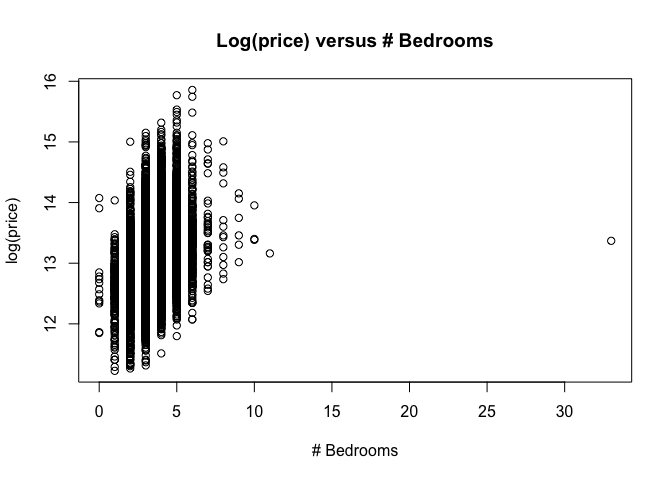
\includegraphics{PriceAnalysis_files/figure-latex/unnamed-chunk-9-1.pdf}
Wow, one of these houses has more than thirty bedrooms.

\begin{Shaded}
\begin{Highlighting}[]
\KeywordTok{max}\NormalTok{(kc3}\OperatorTok{$}\NormalTok{bedrooms)}
\end{Highlighting}
\end{Shaded}

\begin{verbatim}
## [1] 33
\end{verbatim}

Who needs 33 bedrooms?!? Is this a hotel? Let's plot this again without
this data point to see if there is a trend.

\begin{Shaded}
\begin{Highlighting}[]
\KeywordTok{plot}\NormalTok{(kc3}\OperatorTok{$}\NormalTok{bedrooms[kc3}\OperatorTok{$}\NormalTok{bedrooms}\OperatorTok{<}\DecValTok{33}\NormalTok{], }\KeywordTok{log}\NormalTok{(kc3}\OperatorTok{$}\NormalTok{price[kc3}\OperatorTok{$}\NormalTok{bedrooms}\OperatorTok{<}\DecValTok{33}\NormalTok{]),}\DataTypeTok{xlab=}\StringTok{"# Bedrooms"}\NormalTok{,}\DataTypeTok{ylab=}\StringTok{"log(price)"}\NormalTok{, }\DataTypeTok{main=}\StringTok{"Log(price) versus # Bedrooms"}\NormalTok{ )}
\end{Highlighting}
\end{Shaded}

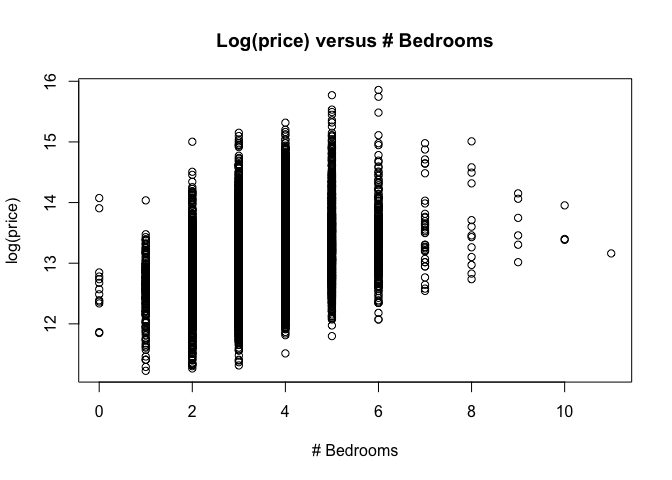
\includegraphics{PriceAnalysis_files/figure-latex/unnamed-chunk-11-1.pdf}
It looks like it generally increases, although there is a lot of
variance. Let's use a box plot:

\begin{Shaded}
\begin{Highlighting}[]
\KeywordTok{plot}\NormalTok{(}\KeywordTok{as.factor}\NormalTok{(kc3}\OperatorTok{$}\NormalTok{bedrooms), }\KeywordTok{log}\NormalTok{(kc3}\OperatorTok{$}\NormalTok{price),}\DataTypeTok{xlab=}\StringTok{"# Bedrooms"}\NormalTok{,}\DataTypeTok{ylab=}\StringTok{"log(price)"}\NormalTok{, }\DataTypeTok{main=}\StringTok{"Log(price) versus # Bedrooms"}\NormalTok{ )}
\end{Highlighting}
\end{Shaded}

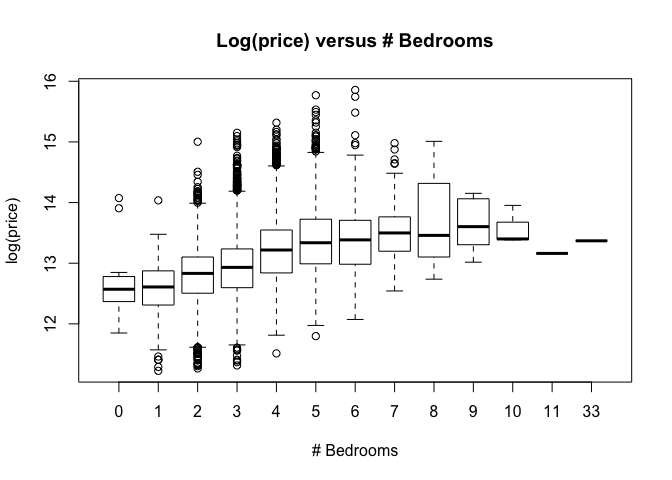
\includegraphics{PriceAnalysis_files/figure-latex/unnamed-chunk-12-1.pdf}
The trend is much clearer here.

\subsubsection{Price versus bathrooms}\label{price-versus-bathrooms}

\begin{Shaded}
\begin{Highlighting}[]
\KeywordTok{plot}\NormalTok{(}\KeywordTok{as.factor}\NormalTok{(kc3}\OperatorTok{$}\NormalTok{bathrooms), }\KeywordTok{log}\NormalTok{(kc3}\OperatorTok{$}\NormalTok{price),}\DataTypeTok{xlab=}\StringTok{"# Bathrooms"}\NormalTok{,}\DataTypeTok{ylab=}\StringTok{"log(price)"}\NormalTok{, }\DataTypeTok{main=}\StringTok{"Log(price) versus # Bathrooms"}\NormalTok{)}
\end{Highlighting}
\end{Shaded}

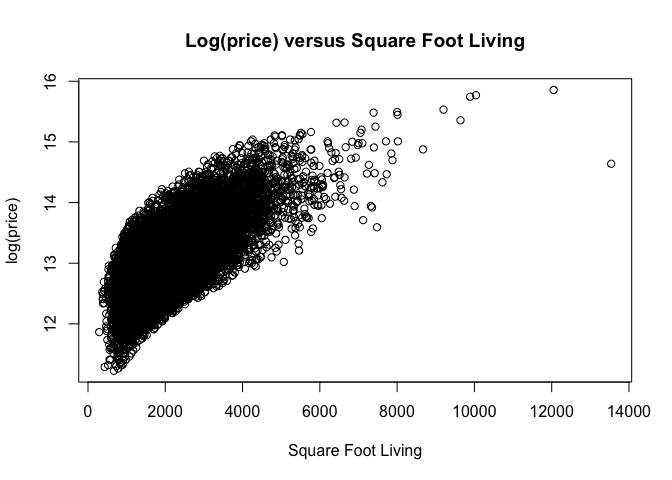
\includegraphics{PriceAnalysis_files/figure-latex/unnamed-chunk-13-1.pdf}
\#\#\#Price versus Square Foot Living Space

\begin{Shaded}
\begin{Highlighting}[]
\KeywordTok{plot}\NormalTok{(kc3}\OperatorTok{$}\NormalTok{sqft_living, }\KeywordTok{log}\NormalTok{(kc3}\OperatorTok{$}\NormalTok{price),}\DataTypeTok{xlab=}\StringTok{"Square Foot Living"}\NormalTok{,}\DataTypeTok{ylab=}\StringTok{"log(price)"}\NormalTok{, }\DataTypeTok{main=}\StringTok{"Log(price) versus Square Foot Living"}\NormalTok{)}
\end{Highlighting}
\end{Shaded}

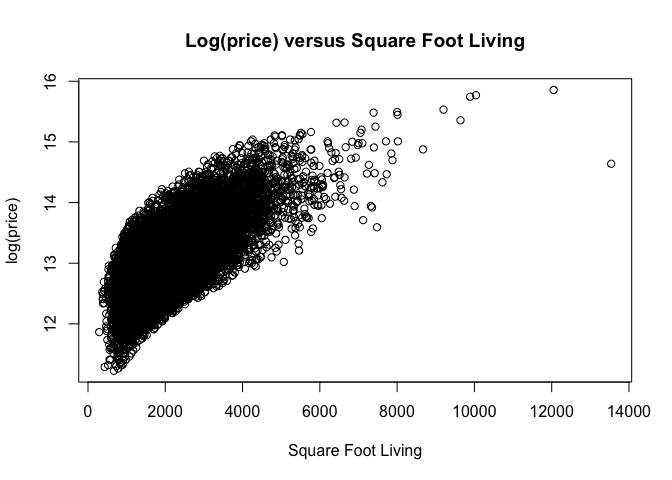
\includegraphics{PriceAnalysis_files/figure-latex/unnamed-chunk-14-1.pdf}
We see that price does increase with square footage, but it doesn't
quite look linear. Let's plot the log-price per square foot:

\begin{Shaded}
\begin{Highlighting}[]
\KeywordTok{plot}\NormalTok{(kc3}\OperatorTok{$}\NormalTok{sqft_living, }\KeywordTok{log}\NormalTok{(kc3}\OperatorTok{$}\NormalTok{price)}\OperatorTok{/}\NormalTok{kc3}\OperatorTok{$}\NormalTok{sqft_living,}\DataTypeTok{xlab=}\StringTok{"Square Foot Living"}\NormalTok{,}\DataTypeTok{ylab=}\StringTok{"Log(Price) Per Square Foot"}\NormalTok{, }\DataTypeTok{main=}\StringTok{"Log(price) versus Square Foot Living"}\NormalTok{)}
\end{Highlighting}
\end{Shaded}

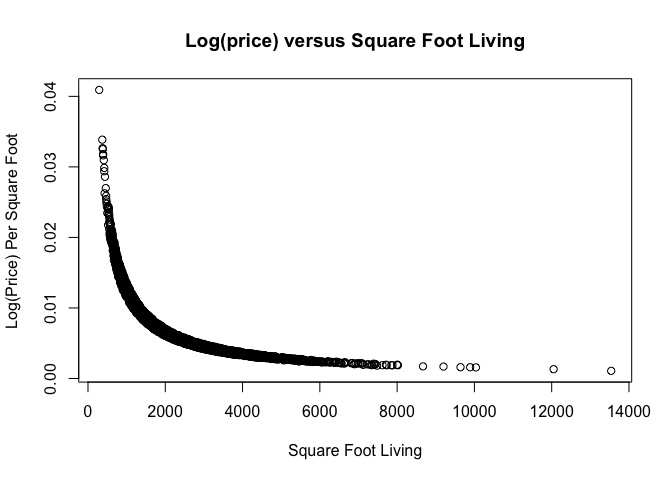
\includegraphics{PriceAnalysis_files/figure-latex/unnamed-chunk-15-1.pdf}
Interesting. The price per square foot decreases with high square
footage. I woud expect the opposite. From the shape of the plot, I think
log(price)/sqft\_living \textasciitilde{} 1/sqrt(sqft\_living)
=\textgreater{} log(price)\textasciitilde{}sqrt(sqft\_living). Let's
see:

\begin{Shaded}
\begin{Highlighting}[]
\KeywordTok{plot}\NormalTok{(}\KeywordTok{sqrt}\NormalTok{(kc3}\OperatorTok{$}\NormalTok{sqft_living), }\KeywordTok{log}\NormalTok{(kc3}\OperatorTok{$}\NormalTok{price),}\DataTypeTok{xlab=}\StringTok{"Square Foot Living"}\NormalTok{,}\DataTypeTok{ylab=}\StringTok{"log(price)"}\NormalTok{, }\DataTypeTok{main=}\StringTok{"Log(price) versus Square Foot Living"}\NormalTok{)}
\end{Highlighting}
\end{Shaded}

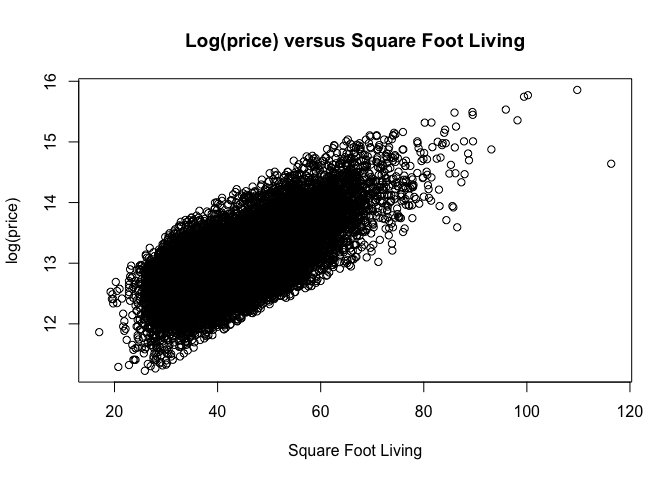
\includegraphics{PriceAnalysis_files/figure-latex/unnamed-chunk-16-1.pdf}
This looks pretty linear, suggesting sqrt(sqft\_living) is a good
feature to use in the linear model. I expect the same holds for the
other square footage units.

\subsubsection{Price versus Floors}\label{price-versus-floors}

\begin{Shaded}
\begin{Highlighting}[]
\KeywordTok{plot}\NormalTok{(}\KeywordTok{as.factor}\NormalTok{(kc3}\OperatorTok{$}\NormalTok{floors), }\KeywordTok{log}\NormalTok{(kc3}\OperatorTok{$}\NormalTok{price),}\DataTypeTok{xlab=}\StringTok{"Number of Floors"}\NormalTok{,}\DataTypeTok{ylab=}\StringTok{"Log(Price)"}\NormalTok{,}\DataTypeTok{main=}\StringTok{"Log(Price) vs # Floors"}\NormalTok{)}
\end{Highlighting}
\end{Shaded}

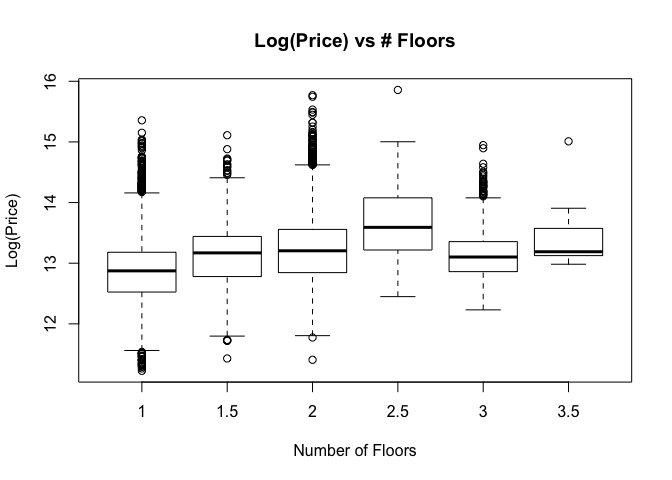
\includegraphics{PriceAnalysis_files/figure-latex/unnamed-chunk-17-1.pdf}
While there seems to be a trend, I think it's largely washed out by the
fluctuation in prices within each floor.

\subsubsection{Price versus Waterfront}\label{price-versus-waterfront}

\begin{Shaded}
\begin{Highlighting}[]
\KeywordTok{plot}\NormalTok{(}\KeywordTok{as.factor}\NormalTok{(kc3}\OperatorTok{$}\NormalTok{waterfront), }\KeywordTok{log}\NormalTok{(kc3}\OperatorTok{$}\NormalTok{price),}\DataTypeTok{xlab=}\StringTok{"?Waterfront"}\NormalTok{,}\DataTypeTok{ylab=}\StringTok{"Log(Price)"}\NormalTok{,}\DataTypeTok{main=}\StringTok{"Log(Price) vs Waterfront"}\NormalTok{)}
\end{Highlighting}
\end{Shaded}

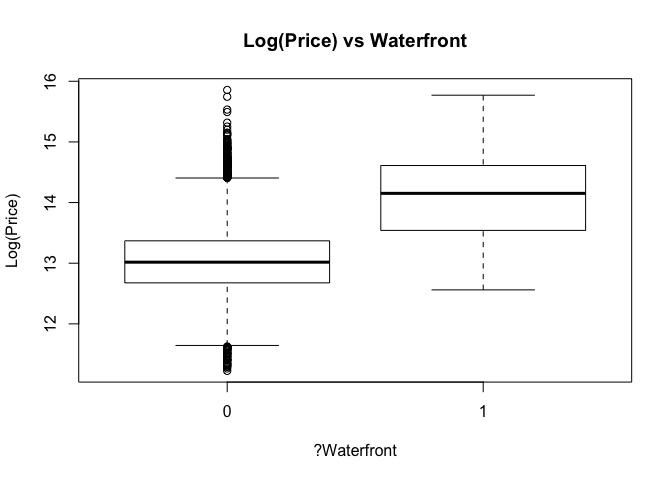
\includegraphics{PriceAnalysis_files/figure-latex/unnamed-chunk-18-1.pdf}
Housing units on the waterfront seem to overall cost more. Are they also
larger? Let's look at sqrt(sqft\_living) against waterfront:

\begin{Shaded}
\begin{Highlighting}[]
\KeywordTok{plot}\NormalTok{(}\KeywordTok{as.factor}\NormalTok{(kc3}\OperatorTok{$}\NormalTok{waterfront), }\KeywordTok{sqrt}\NormalTok{(kc3}\OperatorTok{$}\NormalTok{sqft_living),}\DataTypeTok{xlab=}\StringTok{"?Waterfront"}\NormalTok{,}\DataTypeTok{ylab=}\StringTok{"sqrt(Living Space)"}\NormalTok{,}\DataTypeTok{main=}\StringTok{"sqrt(Living Space) vs Waterfront"}\NormalTok{)}
\end{Highlighting}
\end{Shaded}

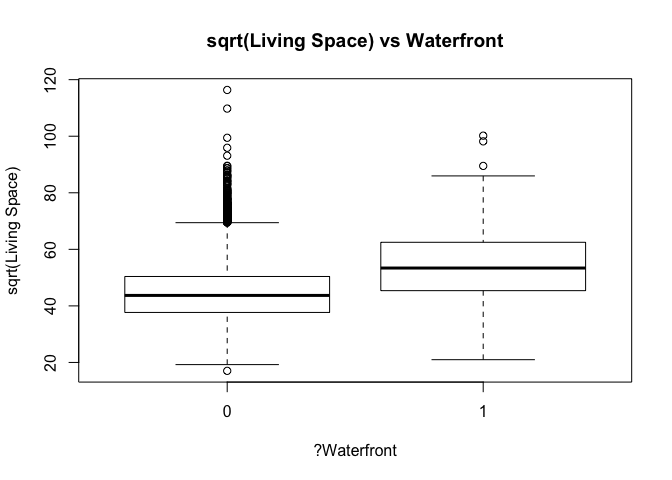
\includegraphics{PriceAnalysis_files/figure-latex/unnamed-chunk-19-1.pdf}
It's hard to say for sure; from the plot it looks like homes on the
waterfront are generally larger, but there is a lot variability.

\subsubsection{Price versus View}\label{price-versus-view}

\begin{Shaded}
\begin{Highlighting}[]
\KeywordTok{plot}\NormalTok{(}\KeywordTok{as.factor}\NormalTok{(kc3}\OperatorTok{$}\NormalTok{view), }\KeywordTok{log}\NormalTok{(kc3}\OperatorTok{$}\NormalTok{price),}\DataTypeTok{xlab=}\StringTok{"?View"}\NormalTok{,}\DataTypeTok{ylab=}\StringTok{"Log(Price)"}\NormalTok{,}\DataTypeTok{main=}\StringTok{"Log(Price) vs View"}\NormalTok{)}
\end{Highlighting}
\end{Shaded}

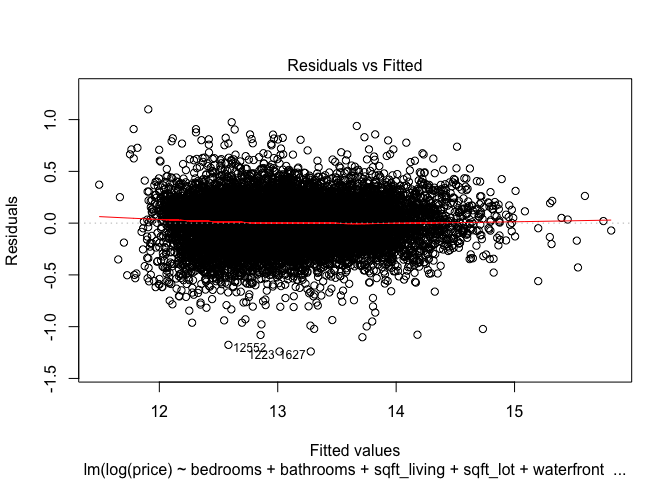
\includegraphics{PriceAnalysis_files/figure-latex/unnamed-chunk-20-1.pdf}

\subsubsection{Price versus Condition}\label{price-versus-condition}

\begin{Shaded}
\begin{Highlighting}[]
\KeywordTok{plot}\NormalTok{(}\KeywordTok{as.factor}\NormalTok{(kc3}\OperatorTok{$}\NormalTok{condition), }\KeywordTok{log}\NormalTok{(kc3}\OperatorTok{$}\NormalTok{price),}\DataTypeTok{xlab=}\StringTok{"Condition"}\NormalTok{,}\DataTypeTok{ylab=}\StringTok{"Log(Price)"}\NormalTok{,}\DataTypeTok{main=}\StringTok{"Log(Price) vs Condition"}\NormalTok{)}
\end{Highlighting}
\end{Shaded}

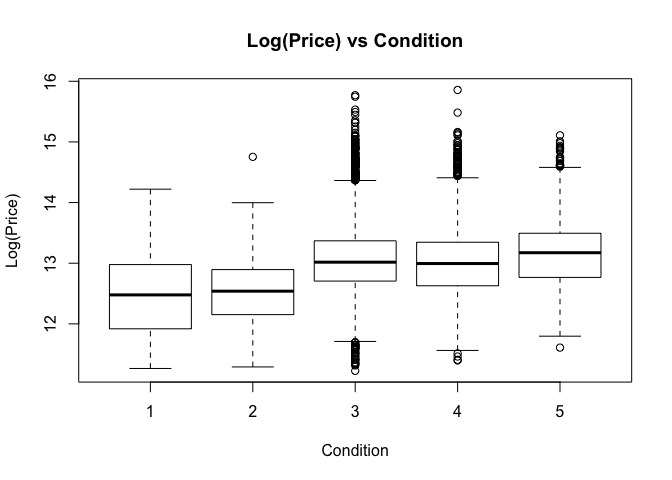
\includegraphics{PriceAnalysis_files/figure-latex/unnamed-chunk-21-1.pdf}
It looks like rather than all the conditions being individually useful,
dividing it by condition \textgreater{} 2 and condition \textless{} 3 is
better.

\begin{Shaded}
\begin{Highlighting}[]
\KeywordTok{plot}\NormalTok{(}\KeywordTok{as.factor}\NormalTok{(kc3}\OperatorTok{$}\NormalTok{condition}\OperatorTok{>}\DecValTok{2}\NormalTok{),}
     \KeywordTok{log}\NormalTok{(kc3}\OperatorTok{$}\NormalTok{price),}\DataTypeTok{xlab=}\StringTok{"?Condition>2"}\NormalTok{,}\DataTypeTok{ylab=}\StringTok{"Log(Price)"}\NormalTok{,}\DataTypeTok{main=}\StringTok{"Log(Price) vs Condition"}\NormalTok{)}
\end{Highlighting}
\end{Shaded}

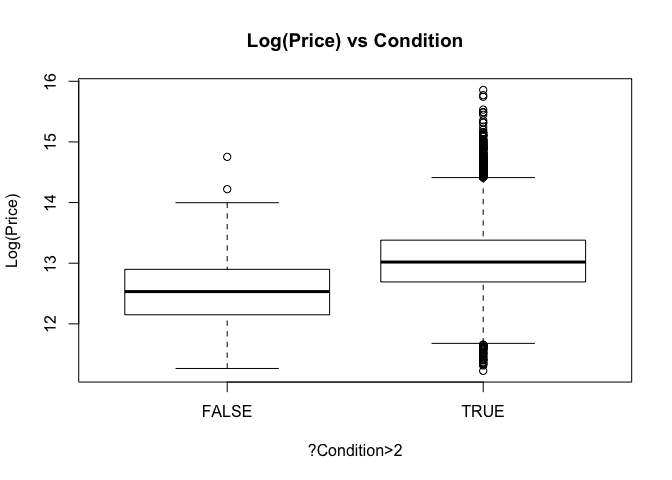
\includegraphics{PriceAnalysis_files/figure-latex/unnamed-chunk-22-1.pdf}

\subsubsection{Price versus Grade}\label{price-versus-grade}

\begin{Shaded}
\begin{Highlighting}[]
\KeywordTok{plot}\NormalTok{(}\KeywordTok{as.factor}\NormalTok{(kc3}\OperatorTok{$}\NormalTok{grade), }\KeywordTok{log}\NormalTok{(kc3}\OperatorTok{$}\NormalTok{price),}\DataTypeTok{xlab=}\StringTok{"Grade"}\NormalTok{,}\DataTypeTok{ylab=}\StringTok{"Log(Price)"}\NormalTok{,}\DataTypeTok{main=}\StringTok{"Log(Price) vs Grade"}\NormalTok{)}
\end{Highlighting}
\end{Shaded}

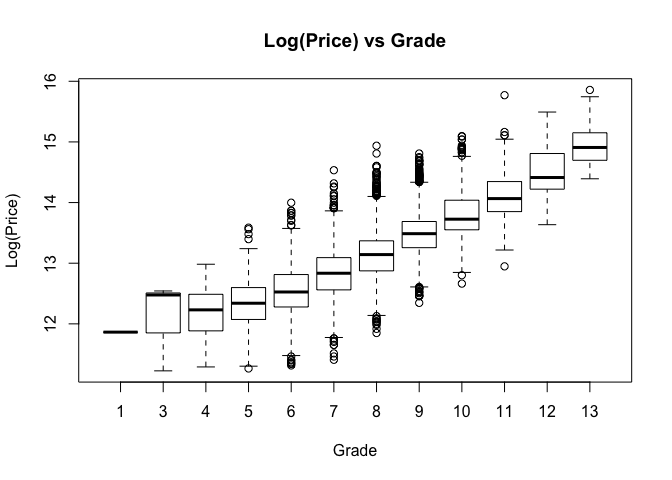
\includegraphics{PriceAnalysis_files/figure-latex/unnamed-chunk-23-1.pdf}

I think it's clear housing units with high grades have higher prices.

\subsubsection{Price versus Year Built}\label{price-versus-year-built}

\begin{Shaded}
\begin{Highlighting}[]
\KeywordTok{plot}\NormalTok{(kc3}\OperatorTok{$}\NormalTok{yr_built, }\KeywordTok{log}\NormalTok{(kc3}\OperatorTok{$}\NormalTok{price),}\DataTypeTok{xlab=}\StringTok{"Year Built"}\NormalTok{,}\DataTypeTok{ylab=}\StringTok{"Log(Price)"}\NormalTok{,}\DataTypeTok{main=}\StringTok{"Log(Price) vs Year Built"}\NormalTok{)}
\end{Highlighting}
\end{Shaded}

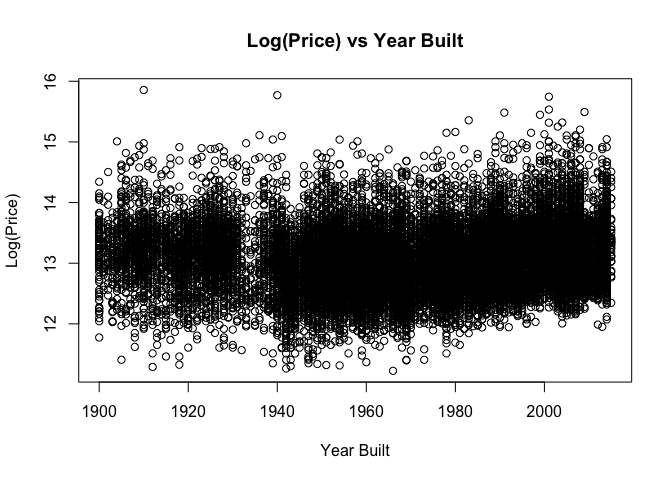
\includegraphics{PriceAnalysis_files/figure-latex/unnamed-chunk-24-1.pdf}

It's hard to establish much of a relationship year.

\subsubsection{Price versus Year
Renovated}\label{price-versus-year-renovated}

\begin{Shaded}
\begin{Highlighting}[]
\KeywordTok{plot}\NormalTok{(kc3}\OperatorTok{$}\NormalTok{yr_renovated, }\KeywordTok{log}\NormalTok{(kc3}\OperatorTok{$}\NormalTok{price),}\DataTypeTok{xlab=}\StringTok{"Year Renovated"}\NormalTok{,}\DataTypeTok{ylab=}\StringTok{"Log(Price)"}\NormalTok{,}\DataTypeTok{main=}\StringTok{"Log(Price) vs Year Renovated"}\NormalTok{)}
\end{Highlighting}
\end{Shaded}

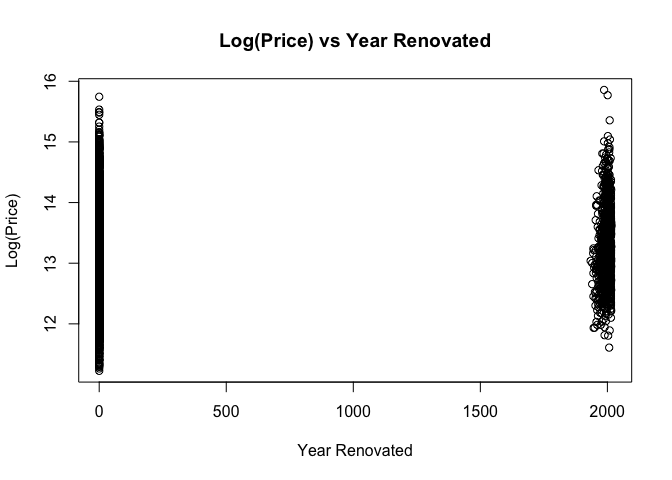
\includegraphics{PriceAnalysis_files/figure-latex/unnamed-chunk-25-1.pdf}
A significant fraction of the points have yr\_renovated = 0, we need to
plot without it:

\begin{Shaded}
\begin{Highlighting}[]
\KeywordTok{plot}\NormalTok{(kc3}\OperatorTok{$}\NormalTok{yr_renovated[kc3}\OperatorTok{$}\NormalTok{yr_renovated}\OperatorTok{>}\DecValTok{0}\NormalTok{], }\KeywordTok{log}\NormalTok{(kc3}\OperatorTok{$}\NormalTok{price[kc3}\OperatorTok{$}\NormalTok{yr_renovated}\OperatorTok{>}\DecValTok{0}\NormalTok{]),}\DataTypeTok{xlab=}\StringTok{"Year Renovated"}\NormalTok{,}\DataTypeTok{ylab=}\StringTok{"Log(Price)"}\NormalTok{,}\DataTypeTok{main=}\StringTok{"Log(Price) vs Year Renovated"}\NormalTok{)}
\end{Highlighting}
\end{Shaded}

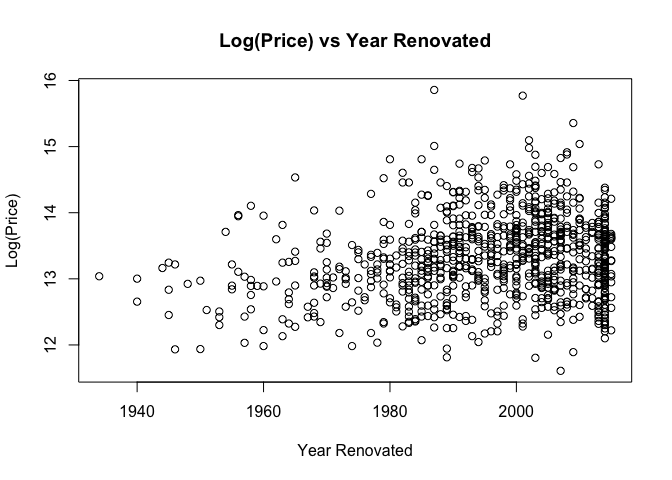
\includegraphics{PriceAnalysis_files/figure-latex/unnamed-chunk-26-1.pdf}

Let's see if simply being renovated is related to price:

\begin{Shaded}
\begin{Highlighting}[]
\KeywordTok{plot}\NormalTok{(}\KeywordTok{as.factor}\NormalTok{(kc3}\OperatorTok{$}\NormalTok{yr_renovated}\OperatorTok{>}\DecValTok{0}\NormalTok{), }\KeywordTok{log}\NormalTok{(kc3}\OperatorTok{$}\NormalTok{price),}\DataTypeTok{xlab=}\StringTok{"?Renovated"}\NormalTok{,}\DataTypeTok{ylab=}\StringTok{"Log(Price)"}\NormalTok{,}\DataTypeTok{main=}\StringTok{"Log(Price) vs ?Renovated"}\NormalTok{)}
\end{Highlighting}
\end{Shaded}

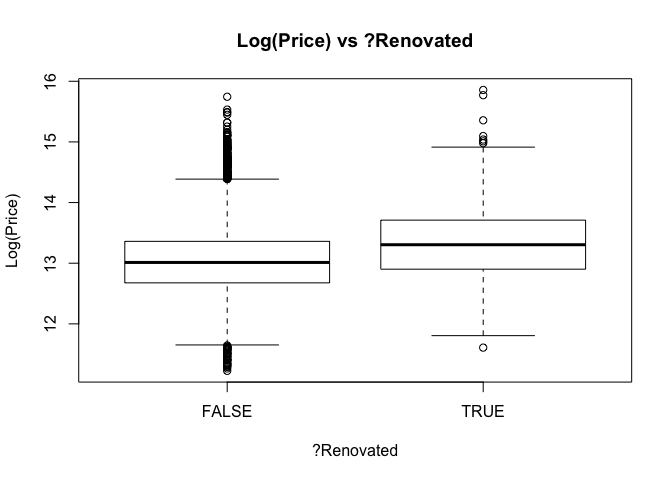
\includegraphics{PriceAnalysis_files/figure-latex/unnamed-chunk-27-1.pdf}

\subsubsection{Price versus Zip Code}\label{price-versus-zip-code}

\begin{Shaded}
\begin{Highlighting}[]
\KeywordTok{plot}\NormalTok{(}\KeywordTok{as.factor}\NormalTok{(kc3}\OperatorTok{$}\NormalTok{zipcode), }\KeywordTok{log}\NormalTok{(kc3}\OperatorTok{$}\NormalTok{price),}\DataTypeTok{xlab=}\StringTok{"Zip Code"}\NormalTok{,}\DataTypeTok{ylab=}\StringTok{"Log(Price)"}\NormalTok{,}\DataTypeTok{main=}\StringTok{"Log(Price) vs Zip Code"}\NormalTok{)}
\end{Highlighting}
\end{Shaded}

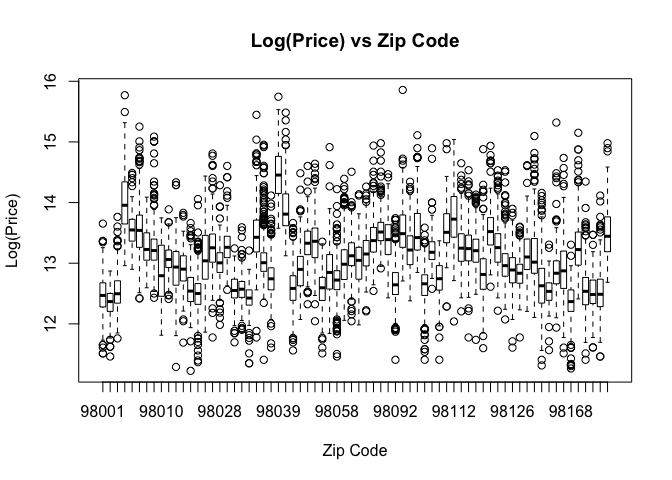
\includegraphics{PriceAnalysis_files/figure-latex/unnamed-chunk-28-1.pdf}

The only sort of trend we might expect is that prices vary across
different ZIP codes, which we do see.

\subsubsection{Price versus Basement}\label{price-versus-basement}

\begin{Shaded}
\begin{Highlighting}[]
\KeywordTok{plot}\NormalTok{(}\KeywordTok{as.factor}\NormalTok{(kc3}\OperatorTok{$}\NormalTok{basement}\OperatorTok{>}\DecValTok{0}\NormalTok{), }\KeywordTok{log}\NormalTok{(kc3}\OperatorTok{$}\NormalTok{price),}\DataTypeTok{xlab=}\StringTok{"?Basement"}\NormalTok{,}\DataTypeTok{ylab=}\StringTok{"Log(Price)"}\NormalTok{,}\DataTypeTok{main=}\StringTok{"Log(Price) vs Presence of basement"}\NormalTok{)}
\end{Highlighting}
\end{Shaded}

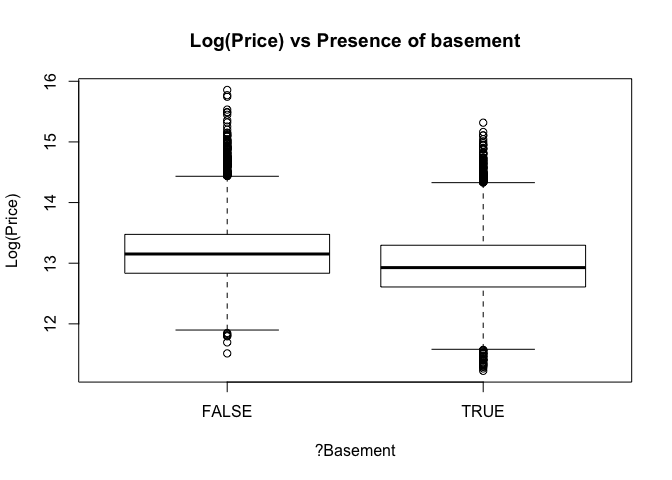
\includegraphics{PriceAnalysis_files/figure-latex/unnamed-chunk-29-1.pdf}

It looks like homes with basements actually tend to cost less, but the
effect is washed out by variability in prices.

\section{Modelling the data}\label{modelling-the-data}

Since housing prices range over several decades, we will take a log of
prices and use a linear model.

\begin{Shaded}
\begin{Highlighting}[]
\NormalTok{fit1 =}\StringTok{ }\KeywordTok{lm}\NormalTok{(}\KeywordTok{log}\NormalTok{(price)}\OperatorTok{~}\NormalTok{.,}\DataTypeTok{data=}\NormalTok{kc3)}
\end{Highlighting}
\end{Shaded}

\begin{Shaded}
\begin{Highlighting}[]
\KeywordTok{summary}\NormalTok{(fit1)}
\end{Highlighting}
\end{Shaded}

\begin{verbatim}
## 
## Call:
## lm(formula = log(price) ~ ., data = kc3)
## 
## Residuals:
##      Min       1Q   Median       3Q      Max 
## -1.63033 -0.09703  0.00825  0.10602  1.04953 
## 
## Coefficients:
##                 Estimate Std. Error t value Pr(>|t|)    
## (Intercept)    1.185e+01  1.456e-01  81.407  < 2e-16 ***
## bedrooms       3.875e-03  1.760e-03   2.202 0.027668 *  
## bathrooms      3.604e-02  3.035e-03  11.872  < 2e-16 ***
## sqft_living    8.553e-05  5.699e-06  15.008  < 2e-16 ***
## sqft_lot       6.047e-07  4.415e-08  13.697  < 2e-16 ***
## floors        -3.016e-02  3.637e-03  -8.294  < 2e-16 ***
## waterfront     4.614e-01  1.624e-02  28.419  < 2e-16 ***
## view           5.836e-02  2.018e-03  28.917  < 2e-16 ***
## condition      5.879e-02  2.214e-03  26.550  < 2e-16 ***
## grade          9.228e-02  2.089e-03  44.169  < 2e-16 ***
## sqft_above     1.186e-04  6.308e-06  18.801  < 2e-16 ***
## yr_built      -3.925e-04  7.462e-05  -5.260 1.45e-07 ***
## yr_renovated   4.155e-05  3.385e-06  12.275  < 2e-16 ***
## zipcode98002  -3.361e-02  1.635e-02  -2.056 0.039790 *  
## zipcode98003   9.199e-03  1.472e-02   0.625 0.531978    
## zipcode98004   1.084e+00  1.443e-02  75.148  < 2e-16 ***
## zipcode98005   7.160e-01  1.743e-02  41.089  < 2e-16 ***
## zipcode98006   6.082e-01  1.304e-02  46.653  < 2e-16 ***
## zipcode98007   6.375e-01  1.841e-02  34.632  < 2e-16 ***
## zipcode98008   6.369e-01  1.473e-02  43.226  < 2e-16 ***
## zipcode98010   2.398e-01  2.097e-02  11.435  < 2e-16 ***
## zipcode98011   4.418e-01  1.645e-02  26.860  < 2e-16 ***
## zipcode98014   2.989e-01  1.955e-02  15.285  < 2e-16 ***
## zipcode98019   3.281e-01  1.664e-02  19.724  < 2e-16 ***
## zipcode98022   3.508e-02  1.571e-02   2.233 0.025584 *  
## zipcode98023  -4.037e-02  1.278e-02  -3.160 0.001579 ** 
## zipcode98024   4.098e-01  2.299e-02  17.822  < 2e-16 ***
## zipcode98027   4.925e-01  1.343e-02  36.676  < 2e-16 ***
## zipcode98028   4.155e-01  1.468e-02  28.296  < 2e-16 ***
## zipcode98029   5.910e-01  1.428e-02  41.386  < 2e-16 ***
## zipcode98030   5.241e-02  1.509e-02   3.474 0.000515 ***
## zipcode98031   6.958e-02  1.480e-02   4.700 2.61e-06 ***
## zipcode98032  -3.944e-02  1.919e-02  -2.055 0.039908 *  
## zipcode98033   7.668e-01  1.322e-02  57.995  < 2e-16 ***
## zipcode98034   5.301e-01  1.255e-02  42.235  < 2e-16 ***
## zipcode98038   1.699e-01  1.240e-02  13.704  < 2e-16 ***
## zipcode98039   1.203e+00  2.815e-02  42.739  < 2e-16 ***
## zipcode98040   8.368e-01  1.500e-02  55.794  < 2e-16 ***
## zipcode98042   5.512e-02  1.253e-02   4.398 1.10e-05 ***
## zipcode98045   3.293e-01  1.583e-02  20.807  < 2e-16 ***
## zipcode98052   6.246e-01  1.249e-02  50.023  < 2e-16 ***
## zipcode98053   5.741e-01  1.353e-02  42.424  < 2e-16 ***
## zipcode98055   1.309e-01  1.491e-02   8.781  < 2e-16 ***
## zipcode98056   3.066e-01  1.338e-02  22.919  < 2e-16 ***
## zipcode98058   1.544e-01  1.302e-02  11.855  < 2e-16 ***
## zipcode98059   3.254e-01  1.300e-02  25.026  < 2e-16 ***
## zipcode98065   3.875e-01  1.443e-02  26.849  < 2e-16 ***
## zipcode98070   3.160e-01  2.019e-02  15.648  < 2e-16 ***
## zipcode98072   4.814e-01  1.489e-02  32.342  < 2e-16 ***
## zipcode98074   5.421e-01  1.326e-02  40.870  < 2e-16 ***
## zipcode98075   5.324e-01  1.404e-02  37.931  < 2e-16 ***
## zipcode98077   4.306e-01  1.659e-02  25.954  < 2e-16 ***
## zipcode98092   2.200e-02  1.389e-02   1.583 0.113369    
## zipcode98102   9.192e-01  2.095e-02  43.871  < 2e-16 ***
## zipcode98103   7.956e-01  1.276e-02  62.358  < 2e-16 ***
## zipcode98105   9.116e-01  1.604e-02  56.821  < 2e-16 ***
## zipcode98106   3.127e-01  1.414e-02  22.122  < 2e-16 ***
## zipcode98107   8.119e-01  1.529e-02  53.098  < 2e-16 ***
## zipcode98108   3.377e-01  1.680e-02  20.100  < 2e-16 ***
## zipcode98109   9.598e-01  2.060e-02  46.601  < 2e-16 ***
## zipcode98112   1.007e+00  1.548e-02  65.056  < 2e-16 ***
## zipcode98115   7.948e-01  1.267e-02  62.732  < 2e-16 ***
## zipcode98116   7.352e-01  1.439e-02  51.104  < 2e-16 ***
## zipcode98117   7.850e-01  1.284e-02  61.158  < 2e-16 ***
## zipcode98118   4.358e-01  1.292e-02  33.733  < 2e-16 ***
## zipcode98119   9.464e-01  1.724e-02  54.885  < 2e-16 ***
## zipcode98122   7.764e-01  1.503e-02  51.652  < 2e-16 ***
## zipcode98125   5.510e-01  1.343e-02  41.019  < 2e-16 ***
## zipcode98126   5.184e-01  1.404e-02  36.921  < 2e-16 ***
## zipcode98133   4.421e-01  1.287e-02  34.336  < 2e-16 ***
## zipcode98136   6.564e-01  1.521e-02  43.145  < 2e-16 ***
## zipcode98144   6.357e-01  1.423e-02  44.678  < 2e-16 ***
## zipcode98146   2.604e-01  1.469e-02  17.728  < 2e-16 ***
## zipcode98148   1.475e-01  2.636e-02   5.595 2.24e-08 ***
## zipcode98155   4.147e-01  1.313e-02  31.593  < 2e-16 ***
## zipcode98166   2.936e-01  1.522e-02  19.292  < 2e-16 ***
## zipcode98168   5.992e-02  1.499e-02   3.999 6.39e-05 ***
## zipcode98177   5.757e-01  1.526e-02  37.728  < 2e-16 ***
## zipcode98178   1.323e-01  1.510e-02   8.765  < 2e-16 ***
## zipcode98188   8.997e-02  1.861e-02   4.835 1.34e-06 ***
## zipcode98198   5.172e-02  1.475e-02   3.506 0.000456 ***
## zipcode98199   8.326e-01  1.454e-02  57.244  < 2e-16 ***
## sqft_living15  8.496e-05  3.321e-06  25.587  < 2e-16 ***
## sqft_lot15     5.742e-08  6.940e-08   0.827 0.408033    
## basement      -4.750e-02  4.897e-03  -9.698  < 2e-16 ***
## ---
## Signif. codes:  0 '***' 0.001 '**' 0.01 '*' 0.05 '.' 0.1 ' ' 1
## 
## Residual standard error: 0.1847 on 21528 degrees of freedom
## Multiple R-squared:  0.8775, Adjusted R-squared:  0.8771 
## F-statistic:  1836 on 84 and 21528 DF,  p-value: < 2.2e-16
\end{verbatim}

\begin{Shaded}
\begin{Highlighting}[]
\KeywordTok{plot}\NormalTok{(fit1)}
\end{Highlighting}
\end{Shaded}

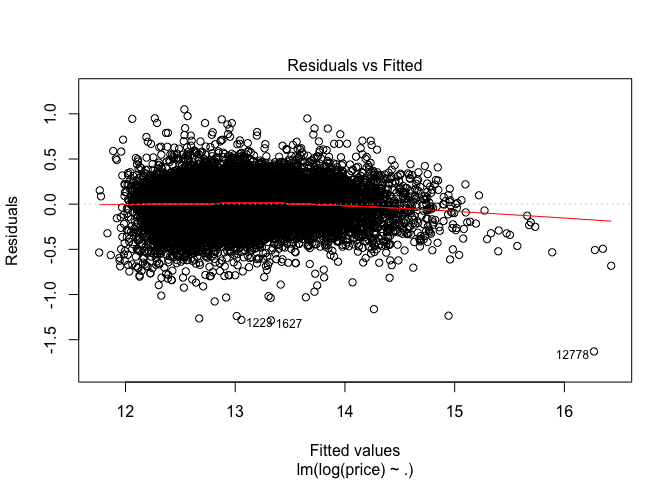
\includegraphics{PriceAnalysis_files/figure-latex/unnamed-chunk-32-1.pdf}
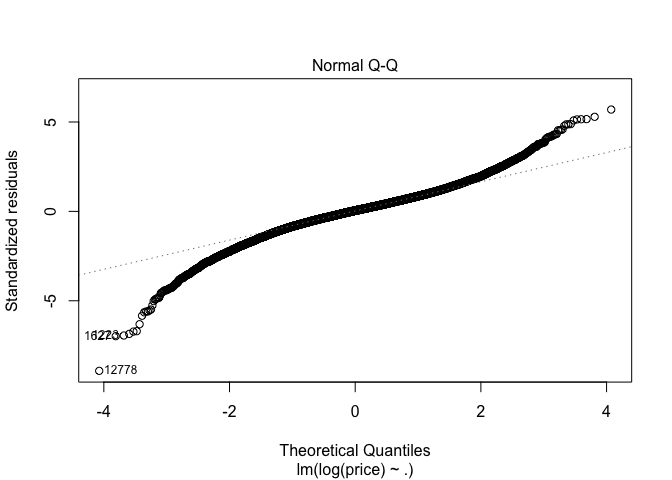
\includegraphics{PriceAnalysis_files/figure-latex/unnamed-chunk-32-2.pdf}
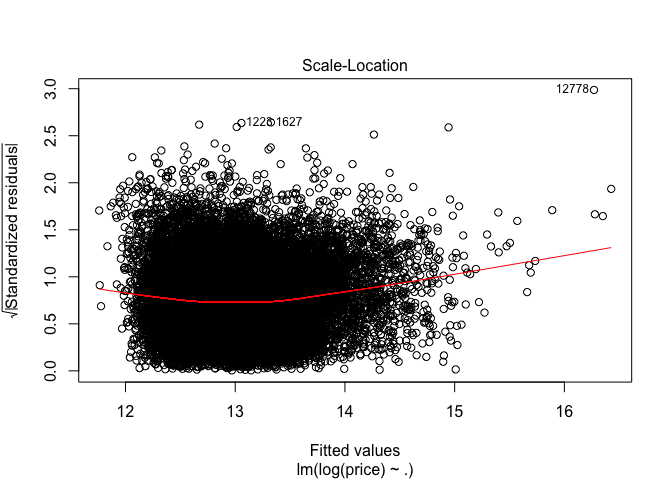
\includegraphics{PriceAnalysis_files/figure-latex/unnamed-chunk-32-3.pdf}
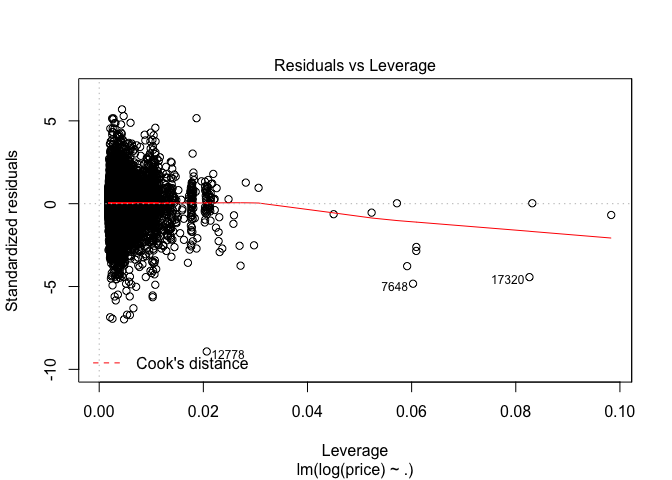
\includegraphics{PriceAnalysis_files/figure-latex/unnamed-chunk-32-4.pdf}
We have an r\^{}2 of about 87\%. Let's modify the model a bit by adding
some features, treating condition and floors as factors, and we'll
remove sqft\_lot\_15.

\begin{Shaded}
\begin{Highlighting}[]
\NormalTok{fit2 =}\StringTok{ }\KeywordTok{update}\NormalTok{(fit1,}\KeywordTok{log}\NormalTok{(price)}\OperatorTok{~}\NormalTok{.}\OperatorTok{+}\KeywordTok{sqrt}\NormalTok{(sqft_living)}\OperatorTok{+}\KeywordTok{sqrt}\NormalTok{(sqft_lot)}\OperatorTok{+}\KeywordTok{sqrt}\NormalTok{(sqft_above)}\OperatorTok{-}\NormalTok{sqft_lot15}\OperatorTok{+}\KeywordTok{as.factor}\NormalTok{(floors)}\OperatorTok{-}\NormalTok{floors}\OperatorTok{-}\NormalTok{condition}\OperatorTok{+}\KeywordTok{as.factor}\NormalTok{(condition)}\OperatorTok{+}\KeywordTok{sqrt}\NormalTok{(sqft_living15 ),}\DataTypeTok{data=}\NormalTok{kc3)}
\KeywordTok{summary}\NormalTok{(fit2)}
\end{Highlighting}
\end{Shaded}

\begin{verbatim}
## 
## Call:
## lm(formula = log(price) ~ bedrooms + bathrooms + sqft_living + 
##     sqft_lot + waterfront + view + grade + sqft_above + yr_built + 
##     yr_renovated + zipcode + sqft_living15 + basement + sqrt(sqft_living) + 
##     sqrt(sqft_lot) + sqrt(sqft_above) + as.factor(floors) + as.factor(condition) + 
##     sqrt(sqft_living15), data = kc3)
## 
## Residuals:
##      Min       1Q   Median       3Q      Max 
## -1.23965 -0.09412  0.00567  0.10072  1.09925 
## 
## Coefficients:
##                         Estimate Std. Error t value Pr(>|t|)    
## (Intercept)            1.050e+01  1.584e-01  66.293  < 2e-16 ***
## bedrooms              -1.151e-02  1.780e-03  -6.467 1.02e-10 ***
## bathrooms              3.127e-02  2.970e-03  10.527  < 2e-16 ***
## sqft_living           -7.016e-05  1.567e-05  -4.477 7.60e-06 ***
## sqft_lot              -2.784e-07  7.748e-08  -3.593 0.000328 ***
## waterfront             4.728e-01  1.577e-02  29.988  < 2e-16 ***
## view                   6.044e-02  1.974e-03  30.617  < 2e-16 ***
## grade                  8.759e-02  2.048e-03  42.780  < 2e-16 ***
## sqft_above             1.214e-05  1.885e-05   0.644 0.519583    
## yr_built              -2.400e-04  7.855e-05  -3.055 0.002250 ** 
## yr_renovated           3.525e-05  3.310e-06  10.651  < 2e-16 ***
## zipcode98002          -5.916e-03  1.590e-02  -0.372 0.709901    
## zipcode98003           1.757e-02  1.429e-02   1.230 0.218631    
## zipcode98004           1.119e+00  1.405e-02  79.634  < 2e-16 ***
## zipcode98005           7.248e-01  1.692e-02  42.827  < 2e-16 ***
## zipcode98006           6.411e-01  1.269e-02  50.523  < 2e-16 ***
## zipcode98007           6.512e-01  1.788e-02  36.415  < 2e-16 ***
## zipcode98008           6.528e-01  1.433e-02  45.542  < 2e-16 ***
## zipcode98010           2.275e-01  2.035e-02  11.176  < 2e-16 ***
## zipcode98011           4.424e-01  1.597e-02  27.705  < 2e-16 ***
## zipcode98014           2.899e-01  1.887e-02  15.361  < 2e-16 ***
## zipcode98019           3.108e-01  1.612e-02  19.280  < 2e-16 ***
## zipcode98022           3.032e-02  1.521e-02   1.993 0.046266 *  
## zipcode98023          -2.650e-02  1.241e-02  -2.136 0.032674 *  
## zipcode98024           4.078e-01  2.229e-02  18.293  < 2e-16 ***
## zipcode98027           4.997e-01  1.302e-02  38.371  < 2e-16 ***
## zipcode98028           4.148e-01  1.426e-02  29.095  < 2e-16 ***
## zipcode98029           5.982e-01  1.390e-02  43.028  < 2e-16 ***
## zipcode98030           5.206e-02  1.464e-02   3.556 0.000378 ***
## zipcode98031           7.331e-02  1.437e-02   5.103 3.37e-07 ***
## zipcode98032          -1.758e-02  1.863e-02  -0.944 0.345352    
## zipcode98033           7.830e-01  1.285e-02  60.919  < 2e-16 ***
## zipcode98034           5.437e-01  1.220e-02  44.575  < 2e-16 ***
## zipcode98038           1.619e-01  1.203e-02  13.454  < 2e-16 ***
## zipcode98039           1.281e+00  2.740e-02  46.751  < 2e-16 ***
## zipcode98040           8.718e-01  1.460e-02  59.726  < 2e-16 ***
## zipcode98042           5.989e-02  1.216e-02   4.926 8.45e-07 ***
## zipcode98045           3.201e-01  1.537e-02  20.826  < 2e-16 ***
## zipcode98052           6.325e-01  1.213e-02  52.146  < 2e-16 ***
## zipcode98053           5.698e-01  1.313e-02  43.397  < 2e-16 ***
## zipcode98055           1.475e-01  1.448e-02  10.186  < 2e-16 ***
## zipcode98056           3.239e-01  1.300e-02  24.919  < 2e-16 ***
## zipcode98058           1.602e-01  1.264e-02  12.677  < 2e-16 ***
## zipcode98059           3.344e-01  1.262e-02  26.498  < 2e-16 ***
## zipcode98065           3.952e-01  1.403e-02  28.166  < 2e-16 ***
## zipcode98070           2.841e-01  1.954e-02  14.542  < 2e-16 ***
## zipcode98072           4.697e-01  1.446e-02  32.480  < 2e-16 ***
## zipcode98074           5.493e-01  1.287e-02  42.665  < 2e-16 ***
## zipcode98075           5.471e-01  1.364e-02  40.123  < 2e-16 ***
## zipcode98077           4.218e-01  1.617e-02  26.077  < 2e-16 ***
## zipcode98092           1.167e-02  1.346e-02   0.867 0.385819    
## zipcode98102           9.792e-01  2.050e-02  47.759  < 2e-16 ***
## zipcode98103           8.524e-01  1.268e-02  67.232  < 2e-16 ***
## zipcode98105           9.550e-01  1.571e-02  60.785  < 2e-16 ***
## zipcode98106           3.691e-01  1.385e-02  26.644  < 2e-16 ***
## zipcode98107           8.737e-01  1.506e-02  58.010  < 2e-16 ***
## zipcode98108           3.771e-01  1.638e-02  23.023  < 2e-16 ***
## zipcode98109           1.004e+00  2.013e-02  49.861  < 2e-16 ***
## zipcode98112           1.054e+00  1.519e-02  69.383  < 2e-16 ***
## zipcode98115           8.322e-01  1.243e-02  66.938  < 2e-16 ***
## zipcode98116           7.767e-01  1.408e-02  55.147  < 2e-16 ***
## zipcode98117           8.335e-01  1.262e-02  66.035  < 2e-16 ***
## zipcode98118           4.795e-01  1.264e-02  37.920  < 2e-16 ***
## zipcode98119           9.904e-01  1.689e-02  58.633  < 2e-16 ***
## zipcode98122           8.231e-01  1.474e-02  55.844  < 2e-16 ***
## zipcode98125           5.809e-01  1.312e-02  44.291  < 2e-16 ***
## zipcode98126           5.712e-01  1.375e-02  41.531  < 2e-16 ***
## zipcode98133           4.774e-01  1.257e-02  37.992  < 2e-16 ***
## zipcode98136           6.988e-01  1.485e-02  47.062  < 2e-16 ***
## zipcode98144           6.849e-01  1.396e-02  49.053  < 2e-16 ***
## zipcode98146           2.916e-01  1.429e-02  20.408  < 2e-16 ***
## zipcode98148           1.711e-01  2.560e-02   6.682 2.42e-11 ***
## zipcode98155           4.363e-01  1.276e-02  34.192  < 2e-16 ***
## zipcode98166           3.080e-01  1.478e-02  20.842  < 2e-16 ***
## zipcode98168           8.997e-02  1.457e-02   6.174 6.77e-10 ***
## zipcode98177           5.917e-01  1.485e-02  39.854  < 2e-16 ***
## zipcode98178           1.597e-01  1.471e-02  10.856  < 2e-16 ***
## zipcode98188           1.061e-01  1.807e-02   5.872 4.38e-09 ***
## zipcode98198           6.839e-02  1.432e-02   4.775 1.81e-06 ***
## zipcode98199           8.684e-01  1.423e-02  61.025  < 2e-16 ***
## sqft_living15         -8.629e-05  2.020e-05  -4.272 1.95e-05 ***
## basement              -2.470e-02  5.410e-03  -4.565 5.03e-06 ***
## sqrt(sqft_living)      1.784e-02  1.637e-03  10.899  < 2e-16 ***
## sqrt(sqft_lot)         6.965e-04  5.198e-05  13.400  < 2e-16 ***
## sqrt(sqft_above)       8.737e-03  1.855e-03   4.710 2.49e-06 ***
## as.factor(floors)1.5   4.107e-04  5.073e-03   0.081 0.935482    
## as.factor(floors)2    -2.856e-02  4.273e-03  -6.684 2.38e-11 ***
## as.factor(floors)2.5  -2.290e-02  1.499e-02  -1.528 0.126440    
## as.factor(floors)3    -1.136e-01  9.346e-03 -12.158  < 2e-16 ***
## as.factor(floors)3.5  -7.259e-02  6.373e-02  -1.139 0.254685    
## as.factor(condition)2  1.322e-01  3.560e-02   3.714 0.000205 ***
## as.factor(condition)3  2.517e-01  3.303e-02   7.621 2.62e-14 ***
## as.factor(condition)4  2.944e-01  3.304e-02   8.911  < 2e-16 ***
## as.factor(condition)5  3.611e-01  3.326e-02  10.859  < 2e-16 ***
## sqrt(sqft_living15)    1.487e-02  1.869e-03   7.959 1.83e-15 ***
## ---
## Signif. codes:  0 '***' 0.001 '**' 0.01 '*' 0.05 '.' 0.1 ' ' 1
## 
## Residual standard error: 0.1791 on 21518 degrees of freedom
## Multiple R-squared:  0.8849, Adjusted R-squared:  0.8844 
## F-statistic:  1759 on 94 and 21518 DF,  p-value: < 2.2e-16
\end{verbatim}

\begin{Shaded}
\begin{Highlighting}[]
\KeywordTok{plot}\NormalTok{(fit2)}
\end{Highlighting}
\end{Shaded}

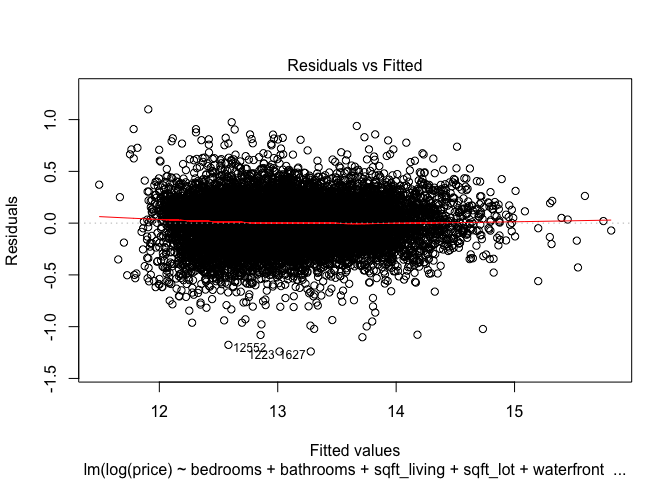
\includegraphics{PriceAnalysis_files/figure-latex/unnamed-chunk-34-1.pdf}
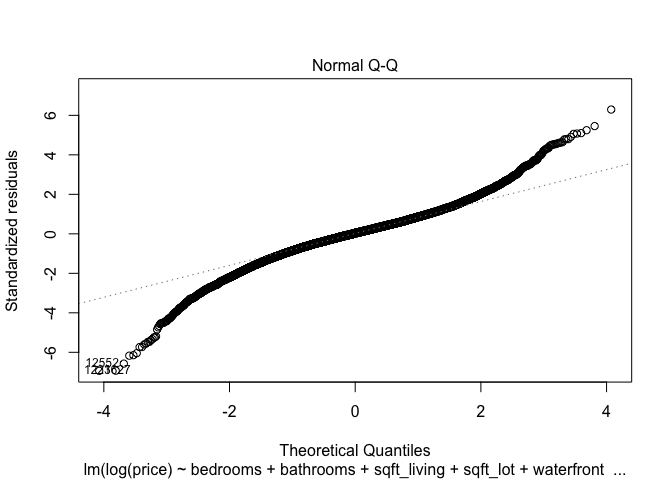
\includegraphics{PriceAnalysis_files/figure-latex/unnamed-chunk-34-2.pdf}
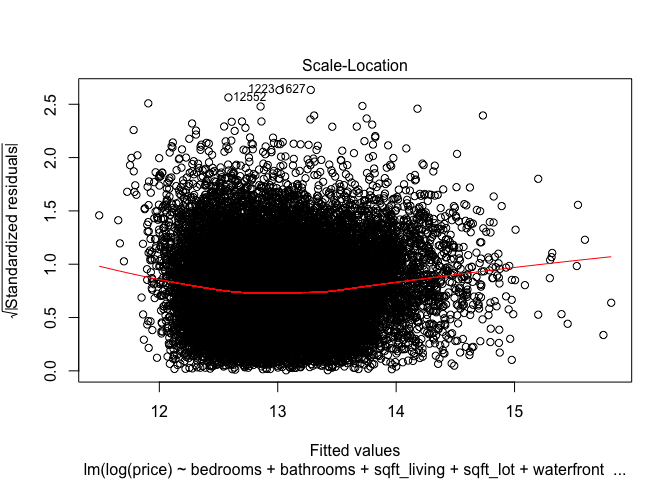
\includegraphics{PriceAnalysis_files/figure-latex/unnamed-chunk-34-3.pdf}
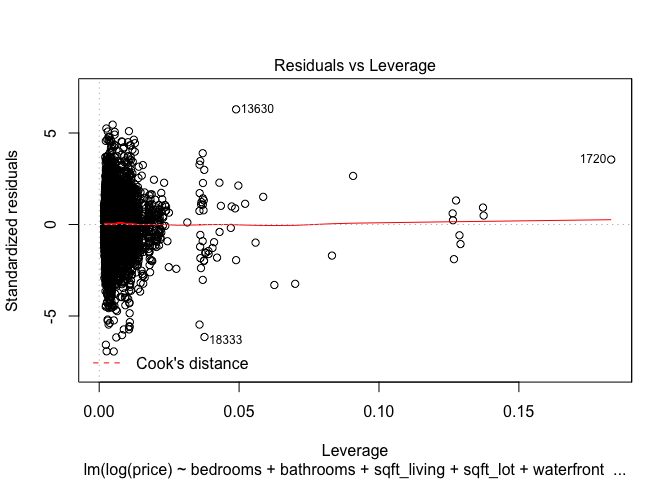
\includegraphics{PriceAnalysis_files/figure-latex/unnamed-chunk-34-4.pdf}
To make sure this model isn't overfitting, we will break up the data
into a training subset and a test subset.

\begin{Shaded}
\begin{Highlighting}[]
\NormalTok{smp_size <-}\StringTok{ }\KeywordTok{floor}\NormalTok{(}\FloatTok{0.8} \OperatorTok{*}\StringTok{ }\KeywordTok{nrow}\NormalTok{(kc3))}
\KeywordTok{set.seed}\NormalTok{(}\DecValTok{1}\NormalTok{)}
\NormalTok{train_ind <-}\StringTok{ }\KeywordTok{sample}\NormalTok{(}\KeywordTok{seq_len}\NormalTok{(}\KeywordTok{nrow}\NormalTok{(kc3)), }\DataTypeTok{size =}\NormalTok{ smp_size)}
\NormalTok{train <-}\StringTok{ }\NormalTok{kc3[train_ind, ]}
\NormalTok{test <-}\StringTok{ }\NormalTok{kc3[}\OperatorTok{-}\NormalTok{train_ind, ]}

\NormalTok{fit2.}\DecValTok{2}\NormalTok{ <-}\StringTok{ }\KeywordTok{update}\NormalTok{(fit2, }\DataTypeTok{data=}\NormalTok{train)}
\end{Highlighting}
\end{Shaded}

\begin{Shaded}
\begin{Highlighting}[]
\KeywordTok{summary}\NormalTok{(fit2.}\DecValTok{2}\NormalTok{)}
\end{Highlighting}
\end{Shaded}

\begin{verbatim}
## 
## Call:
## lm(formula = log(price) ~ bedrooms + bathrooms + sqft_living + 
##     sqft_lot + waterfront + view + grade + sqft_above + yr_built + 
##     yr_renovated + zipcode + sqft_living15 + basement + sqrt(sqft_living) + 
##     sqrt(sqft_lot) + sqrt(sqft_above) + as.factor(floors) + as.factor(condition) + 
##     sqrt(sqft_living15), data = train)
## 
## Residuals:
##      Min       1Q   Median       3Q      Max 
## -1.24086 -0.09458  0.00510  0.10049  1.12976 
## 
## Coefficients:
##                         Estimate Std. Error t value Pr(>|t|)    
## (Intercept)            1.031e+01  1.781e-01  57.899  < 2e-16 ***
## bedrooms              -9.526e-03  1.980e-03  -4.811 1.52e-06 ***
## bathrooms              2.913e-02  3.327e-03   8.756  < 2e-16 ***
## sqft_living           -8.189e-05  1.773e-05  -4.620 3.87e-06 ***
## sqft_lot              -1.665e-07  8.741e-08  -1.905 0.056759 .  
## waterfront             4.390e-01  1.800e-02  24.389  < 2e-16 ***
## view                   6.268e-02  2.224e-03  28.186  < 2e-16 ***
## grade                  8.688e-02  2.299e-03  37.786  < 2e-16 ***
## sqft_above             1.687e-05  2.119e-05   0.796 0.426029    
## yr_built              -1.487e-04  8.819e-05  -1.686 0.091743 .  
## yr_renovated           3.522e-05  3.716e-06   9.478  < 2e-16 ***
## zipcode98002          -8.708e-03  1.780e-02  -0.489 0.624764    
## zipcode98003           1.667e-02  1.621e-02   1.028 0.303837    
## zipcode98004           1.107e+00  1.553e-02  71.327  < 2e-16 ***
## zipcode98005           7.162e-01  1.877e-02  38.166  < 2e-16 ***
## zipcode98006           6.362e-01  1.403e-02  45.328  < 2e-16 ***
## zipcode98007           6.498e-01  2.001e-02  32.473  < 2e-16 ***
## zipcode98008           6.517e-01  1.617e-02  40.306  < 2e-16 ***
## zipcode98010           2.256e-01  2.264e-02   9.962  < 2e-16 ***
## zipcode98011           4.413e-01  1.754e-02  25.153  < 2e-16 ***
## zipcode98014           2.817e-01  2.100e-02  13.410  < 2e-16 ***
## zipcode98019           2.975e-01  1.825e-02  16.295  < 2e-16 ***
## zipcode98022           2.976e-02  1.692e-02   1.759 0.078617 .  
## zipcode98023          -3.625e-02  1.361e-02  -2.664 0.007722 ** 
## zipcode98024           4.090e-01  2.535e-02  16.136  < 2e-16 ***
## zipcode98027           4.938e-01  1.445e-02  34.161  < 2e-16 ***
## zipcode98028           4.066e-01  1.588e-02  25.604  < 2e-16 ***
## zipcode98029           5.966e-01  1.529e-02  39.012  < 2e-16 ***
## zipcode98030           5.068e-02  1.649e-02   3.074 0.002117 ** 
## zipcode98031           7.170e-02  1.598e-02   4.486 7.31e-06 ***
## zipcode98032          -2.650e-02  2.080e-02  -1.274 0.202671    
## zipcode98033           7.793e-01  1.416e-02  55.025  < 2e-16 ***
## zipcode98034           5.413e-01  1.361e-02  39.777  < 2e-16 ***
## zipcode98038           1.615e-01  1.342e-02  12.032  < 2e-16 ***
## zipcode98039           1.276e+00  2.917e-02  43.737  < 2e-16 ***
## zipcode98040           8.640e-01  1.632e-02  52.942  < 2e-16 ***
## zipcode98042           6.191e-02  1.342e-02   4.614 3.98e-06 ***
## zipcode98045           3.079e-01  1.747e-02  17.625  < 2e-16 ***
## zipcode98052           6.348e-01  1.346e-02  47.164  < 2e-16 ***
## zipcode98053           5.734e-01  1.471e-02  38.993  < 2e-16 ***
## zipcode98055           1.552e-01  1.612e-02   9.627  < 2e-16 ***
## zipcode98056           3.143e-01  1.447e-02  21.725  < 2e-16 ***
## zipcode98058           1.580e-01  1.393e-02  11.340  < 2e-16 ***
## zipcode98059           3.267e-01  1.405e-02  23.249  < 2e-16 ***
## zipcode98065           3.922e-01  1.546e-02  25.371  < 2e-16 ***
## zipcode98070           2.783e-01  2.175e-02  12.795  < 2e-16 ***
## zipcode98072           4.685e-01  1.609e-02  29.122  < 2e-16 ***
## zipcode98074           5.474e-01  1.428e-02  38.329  < 2e-16 ***
## zipcode98075           5.420e-01  1.532e-02  35.375  < 2e-16 ***
## zipcode98077           4.170e-01  1.779e-02  23.439  < 2e-16 ***
## zipcode98092           1.168e-02  1.481e-02   0.789 0.430272    
## zipcode98102           9.911e-01  2.323e-02  42.656  < 2e-16 ***
## zipcode98103           8.380e-01  1.405e-02  59.646  < 2e-16 ***
## zipcode98105           9.448e-01  1.745e-02  54.158  < 2e-16 ***
## zipcode98106           3.587e-01  1.545e-02  23.218  < 2e-16 ***
## zipcode98107           8.723e-01  1.698e-02  51.363  < 2e-16 ***
## zipcode98108           3.763e-01  1.816e-02  20.717  < 2e-16 ***
## zipcode98109           1.008e+00  2.319e-02  43.455  < 2e-16 ***
## zipcode98112           1.046e+00  1.726e-02  60.603  < 2e-16 ***
## zipcode98115           8.262e-01  1.383e-02  59.743  < 2e-16 ***
## zipcode98116           7.754e-01  1.560e-02  49.690  < 2e-16 ***
## zipcode98117           8.262e-01  1.395e-02  59.240  < 2e-16 ***
## zipcode98118           4.786e-01  1.399e-02  34.212  < 2e-16 ***
## zipcode98119           9.800e-01  1.845e-02  53.105  < 2e-16 ***
## zipcode98122           8.213e-01  1.640e-02  50.083  < 2e-16 ***
## zipcode98125           5.848e-01  1.458e-02  40.108  < 2e-16 ***
## zipcode98126           5.586e-01  1.510e-02  36.995  < 2e-16 ***
## zipcode98133           4.717e-01  1.392e-02  33.891  < 2e-16 ***
## zipcode98136           6.974e-01  1.641e-02  42.498  < 2e-16 ***
## zipcode98144           6.886e-01  1.553e-02  44.345  < 2e-16 ***
## zipcode98146           2.999e-01  1.576e-02  19.026  < 2e-16 ***
## zipcode98148           1.653e-01  2.943e-02   5.618 1.96e-08 ***
## zipcode98155           4.309e-01  1.415e-02  30.462  < 2e-16 ***
## zipcode98166           3.003e-01  1.657e-02  18.123  < 2e-16 ***
## zipcode98168           8.356e-02  1.633e-02   5.117 3.13e-07 ***
## zipcode98177           5.903e-01  1.661e-02  35.546  < 2e-16 ***
## zipcode98178           1.427e-01  1.647e-02   8.664  < 2e-16 ***
## zipcode98188           9.907e-02  2.043e-02   4.849 1.25e-06 ***
## zipcode98198           7.387e-02  1.586e-02   4.659 3.20e-06 ***
## zipcode98199           8.674e-01  1.579e-02  54.947  < 2e-16 ***
## sqft_living15         -7.768e-05  2.234e-05  -3.477 0.000508 ***
## basement              -2.523e-02  6.075e-03  -4.154 3.28e-05 ***
## sqrt(sqft_living)      1.892e-02  1.841e-03  10.277  < 2e-16 ***
## sqrt(sqft_lot)         6.603e-04  5.852e-05  11.282  < 2e-16 ***
## sqrt(sqft_above)       8.121e-03  2.078e-03   3.908 9.35e-05 ***
## as.factor(floors)1.5   4.254e-03  5.711e-03   0.745 0.456323    
## as.factor(floors)2    -2.782e-02  4.795e-03  -5.801 6.72e-09 ***
## as.factor(floors)2.5  -2.151e-02  1.673e-02  -1.286 0.198574    
## as.factor(floors)3    -1.160e-01  1.041e-02 -11.144  < 2e-16 ***
## as.factor(floors)3.5  -1.082e-01  8.107e-02  -1.334 0.182086    
## as.factor(condition)2  1.577e-01  4.014e-02   3.928 8.60e-05 ***
## as.factor(condition)3  2.756e-01  3.716e-02   7.415 1.27e-13 ***
## as.factor(condition)4  3.210e-01  3.718e-02   8.635  < 2e-16 ***
## as.factor(condition)5  3.882e-01  3.743e-02  10.372  < 2e-16 ***
## sqrt(sqft_living15)    1.423e-02  2.072e-03   6.864 6.92e-12 ***
## ---
## Signif. codes:  0 '***' 0.001 '**' 0.01 '*' 0.05 '.' 0.1 ' ' 1
## 
## Residual standard error: 0.1799 on 17195 degrees of freedom
## Multiple R-squared:  0.8837, Adjusted R-squared:  0.8831 
## F-statistic:  1390 on 94 and 17195 DF,  p-value: < 2.2e-16
\end{verbatim}

Let's evaluate the performance by looking at r\^{}2 and RSS.

\begin{Shaded}
\begin{Highlighting}[]
\NormalTok{RSS.train <-}\StringTok{ }\KeywordTok{sum}\NormalTok{((}\KeywordTok{predict}\NormalTok{(fit2.}\DecValTok{2}\NormalTok{,train) }\OperatorTok{-}\StringTok{ }\KeywordTok{log}\NormalTok{(train}\OperatorTok{$}\NormalTok{price) )}\OperatorTok{^}\DecValTok{2}\NormalTok{ )}
\NormalTok{TSS.train <-}\StringTok{ }\KeywordTok{sum}\NormalTok{((}\KeywordTok{mean}\NormalTok{(}\KeywordTok{log}\NormalTok{(train}\OperatorTok{$}\NormalTok{price)) }\OperatorTok{-}\StringTok{ }\KeywordTok{log}\NormalTok{(train}\OperatorTok{$}\NormalTok{price) )}\OperatorTok{^}\DecValTok{2}\NormalTok{) }
\KeywordTok{cat}\NormalTok{(}\StringTok{"R-squared for train data: "}\NormalTok{,}\DecValTok{1}\OperatorTok{-}\NormalTok{RSS.train}\OperatorTok{/}\NormalTok{TSS.train)}
\end{Highlighting}
\end{Shaded}

\begin{verbatim}
## R-squared for train data:  0.8837133
\end{verbatim}

\begin{Shaded}
\begin{Highlighting}[]
\NormalTok{RSS.test <-}\StringTok{ }\KeywordTok{sum}\NormalTok{((}\KeywordTok{predict}\NormalTok{(fit2.}\DecValTok{2}\NormalTok{,test) }\OperatorTok{-}\StringTok{ }\KeywordTok{log}\NormalTok{(test}\OperatorTok{$}\NormalTok{price) )}\OperatorTok{^}\DecValTok{2}\NormalTok{ )}
\NormalTok{TSS.test <-}\StringTok{ }\KeywordTok{sum}\NormalTok{((}\KeywordTok{mean}\NormalTok{(}\KeywordTok{log}\NormalTok{(test}\OperatorTok{$}\NormalTok{price)) }\OperatorTok{-}\StringTok{ }\KeywordTok{log}\NormalTok{(test}\OperatorTok{$}\NormalTok{price) )}\OperatorTok{^}\DecValTok{2}\NormalTok{) }
\KeywordTok{cat}\NormalTok{(}\StringTok{"R-squared for test data: "}\NormalTok{,}\DecValTok{1}\OperatorTok{-}\NormalTok{RSS.test}\OperatorTok{/}\NormalTok{TSS.test)}
\end{Highlighting}
\end{Shaded}

\begin{verbatim}
## R-squared for test data:  0.88838
\end{verbatim}

\begin{Shaded}
\begin{Highlighting}[]
\NormalTok{RSS.total <-}\StringTok{ }\KeywordTok{sum}\NormalTok{((}\KeywordTok{predict}\NormalTok{(fit2.}\DecValTok{2}\NormalTok{,kc3) }\OperatorTok{-}\StringTok{ }\KeywordTok{log}\NormalTok{(kc3}\OperatorTok{$}\NormalTok{price) )}\OperatorTok{^}\DecValTok{2}\NormalTok{ )}
\NormalTok{TSS.total <-}\StringTok{ }\KeywordTok{sum}\NormalTok{((}\KeywordTok{mean}\NormalTok{(}\KeywordTok{log}\NormalTok{(kc3}\OperatorTok{$}\NormalTok{price)) }\OperatorTok{-}\StringTok{ }\KeywordTok{log}\NormalTok{(kc3}\OperatorTok{$}\NormalTok{price) )}\OperatorTok{^}\DecValTok{2}\NormalTok{) }
\KeywordTok{cat}\NormalTok{(}\StringTok{"R-squared for all data: "}\NormalTok{,}\DecValTok{1}\OperatorTok{-}\NormalTok{RSS.total}\OperatorTok{/}\NormalTok{TSS.total)}
\end{Highlighting}
\end{Shaded}

\begin{verbatim}
## R-squared for all data:  0.8846585
\end{verbatim}

\begin{Shaded}
\begin{Highlighting}[]
\KeywordTok{cat}\NormalTok{(}\StringTok{"RMS for all data: "}\NormalTok{,}\KeywordTok{sqrt}\NormalTok{(}\KeywordTok{mean}\NormalTok{((}\KeywordTok{predict}\NormalTok{(fit2.}\DecValTok{2}\NormalTok{,kc3) }\OperatorTok{-}\StringTok{ }\KeywordTok{log}\NormalTok{(kc3}\OperatorTok{$}\NormalTok{price) )}\OperatorTok{^}\DecValTok{2}\NormalTok{ )))}
\end{Highlighting}
\end{Shaded}

\begin{verbatim}
## RMS for all data:  0.1788683
\end{verbatim}

The model is performing well with an R-squared of about 88\% for all the
data as well as the training and test subsets. Our mean squared error is
about 0.18. Since we predicted the log of price, we exponentiate our
prediction to get actual price, and our error becomes multiplicative,
i.e.~exp(log(price)+-RMSE) = exp(+-RMSE)*price. Since exp(+RMSE) is
about 1.2 and exp(-RMSE) is about 0.84, we're overestimating or
underestimating price by about 20\% on average.

\begin{Shaded}
\begin{Highlighting}[]
\KeywordTok{exp}\NormalTok{(}\OperatorTok{-}\FloatTok{0.18}\NormalTok{)}
\end{Highlighting}
\end{Shaded}

\begin{verbatim}
## [1] 0.8352702
\end{verbatim}


\end{document}
